\documentclass[12pt,a4paper]{tufte-handout}

\title{Work and Energy\thanks{Draft version as of \today}}

\author[dishajk]{Disha Kuzhively}

%\date{28 March 2010} % without \date command, current date is supplied

%\geometry{showframe} % display margins for debugging page layout

\usepackage{graphicx} % allow embedded images
  \setkeys{Gin}{width=\linewidth,totalheight=\textheight,keepaspectratio}
  \graphicspath{{graphics/}} % set of paths to search for images
\usepackage{amsmath}  % extended mathematics
\usepackage{booktabs} % book-quality tables
% \usepackage{units}    % non-stacked fractions and better unit spacing
\usepackage{multicol} % multiple column layout facilities
\usepackage{fancyvrb} % extended verbatim environments
  \fvset{fontsize=\normalsize}% default font size for fancy-verbatim environments
\usepackage{url}
\usepackage{hyperref}
\usepackage{tikz}
\usetikzlibrary{calc,patterns}
\usepackage[none]{hyphenat}
\usepackage{svg}
\usepackage{siunitx}
\usepackage{array}
\usepackage{float}
% Standardize command font styles and environments
\newcommand{\doccmd}[1]{\texttt{\textbackslash#1}}% command name -- adds backslash automatically
\newcommand{\docopt}[1]{\ensuremath{\langle}\textrm{\textit{#1}}\ensuremath{\rangle}}% optional command argument
\newcommand{\docarg}[1]{\textrm{\textit{#1}}}% (required) command argument
\newcommand{\docenv}[1]{\textsf{#1}}% environment name
\newcommand{\docpkg}[1]{\texttt{#1}}% package name
\newcommand{\doccls}[1]{\texttt{#1}}% document class name
\newcommand{\docclsopt}[1]{\texttt{#1}}% document class option name
\newenvironment{docspec}{\begin{quote}\noindent}{\end{quote}}% command specification environment

\newcommand{\hertz}{Hz}

\tikzset{
    pencil/.pic={
        \pgfmathsetmacro{\l}{3}
        \pgfmathsetmacro{\w}{\l/10}
        % Pencil body
        \fill[orange!80!yellow] (0,0) rectangle (\l,\w);
        % Wooden sharpened part
        \fill[brown!30] (\l,0) -- ({7*\l/6},\w/2) -- (\l,\w) -- cycle;
        
        \fill[black] ({7*\l/6},{\w/2}) -- ($({7*\l/6},{\w/2})!0.3!(\l,\w)$) --($({7*\l/6},{\w/2})!0.3!(\l,0)$) --cycle;
        % Edge lines

        \draw (0,0) rectangle (\l,\w);

        \draw (\l,0) -- ({7*\l/6},\w/2) -- (\l,\w);
        \fill[pink!60,draw=black] (-\w,0) rectangle (0,\w);
        \fill[gray!50, draw=black] (-\w/3,0) rectangle (0,\w);
    },
    speaker/.pic={
        \draw (-1,-1) --++ (0.5,0) --++ (1.5,-1)--++(0,3)--++(-1.5,-1)--++(-0.5,0);
        \node[text width=2cm] at (0,-.5) {Source of sound}; 
    }
}

\begin{document}
% \printclassoptions

\maketitle% this prints the handout title, author, and date

\begin{abstract}
\noindent
This article was prepared by the author to serve as a draft for TNSCERT class 7 chapter on the concept of Work and Energy during the the Tamil Nadu Curriculum Framing (TNCF) workshop that was held in Asha Nivas, Chennai  from 13-11-2025 to 15-11-2025, 09-03-2026 to 10-03-2026, and 27-04-2026 to 30-04-2026.

The right side margin of each page contains notes for teachers, and prompts to activities that the teacher can initiate in the classroom.

% This draft assumes that the student knows: Force effect on motion, heat (thermal energy), 

% Cant assume understanding of difference between distance and displacement, acceleration due to gravity, 

\begin{quotation}
Draft Syllabus\cite{draftSyllabus}:

C 1.11: Understands and calculates work and energy, identifies different forms and sources of energy, observes and represents energy changes in real-life situations.

Work and Energy:
Work: Concept and definition of work in science - quantification of work done by a steady force, Simple numerical problems, SI Unit of Work (Joule)

C 1.12: Applies scientific knowledge and uses appropriate scientific vocabulary to communicate ideas and to promote responsible use of energy.

Energy: Concept and definition of energy, different forms of energy, conversion of energy, energy flow in daily life systems, useful and wasted forms of energy, law of conservation of energy, sources of energy - renewable and non-renewable energy sources-conservation
\end{quotation}
\end{abstract}
In earlier lessons, we learned that a force is needed to start motion, stop motion, change speed, or change the direction of motion.

Let us do a simple activity. Place a book on the desk and push it slowly so that it slides at a steady speed. By pushing slowly, we are trying to apply a constant force to move the book. In everyday language, we say that we are doing some \emph{work}. If we push the same book a longer distance or if we are pushing a heavier stack of books the same distance, we are doing more work than we did initially.

\begin{figure}
  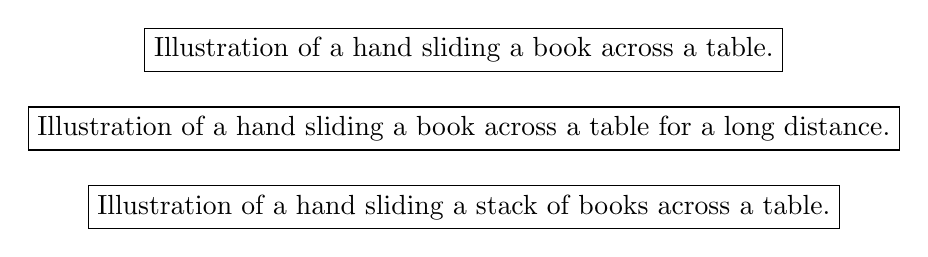
\begin{tikzpicture}
    \node[draw] at (0,0) {Illustration of a hand sliding a book across a table.};
    \node[draw] at (-90:1) {Illustration of a hand sliding a book across a table for a long distance.};
    \node[draw] at (-90:2) {Illustration of a hand sliding a stack of books across a table.};
  \end{tikzpicture}
  \caption{Sliding a book across a table.}
  \label{fig:slidingBook}
\end{figure}
From this, we can see that the work done depends on two things:
\begin{enumerate}
\item how much force is applied, and
\item how far the object moves.
\end{enumerate}
\newthought{Exercise: }Write down all the work that you do in your daily life.
When a constant force $(F)$ moves an object through some dsitance $(d)$ in the same direction as the force, the work done $(W)$ is defined as:
\begin{equation}\label{eq:workDef}
W = F \times d
\end{equation}
The SI unit of work is Joule $(\unit\joule)$, named for James Prescott Joule, an English scientist of the 1800s.

The SI unit of force is Newton $(\unit\newton)$ and the SI unit of distance is metre $(\unit\metre)$. This makes
\begin{equation}
  1~ \unit\joule = 1~ \unit\newton\times 1~\unit\metre  
\end{equation}
\newthought{Example:} If we apply a force of $10~\unit\newton$ to push the book a distance of $2~\unit\metre$, the work done $= 10~\unit\newton \times 2~\unit\metre = 20~\unit\joule$.

\newthought{Question:} In which of the following cases is work being done? In which of these cases are we applying force but there is no movement?
\begin{enumerate}
\item Holding a heavy bag 
\item Pushing a wall 
\item Climbing stairs 
\item Kicking a ball 
\item Sitting and reading
\end{enumerate}
Remember that we are not concerned here with the common meaning of the word ``work,” which implies that any physical or mental labor is work. We are only concerned with work where there is a force acting on an object and the object moves in the direction of the force.

\newthought{Question:} Why is pushing a wall not considered work in physics?
\subsection{When is work done zero?}
From the definition of work done (Equation \ref{eq:workDef}), we can see that work done is zero if no force is applied by the agent , i.e., $F = 0$. If the object does not move, $d = 0$, then no work done even if you are applying a force. For example, if you push a wall and it does not move, the work done is zero.

Work is done only when the force acts in the same direction as the movement. If the force acts in a direction perpendicular (at a right angle) to the movement, then the work done by that force is zero.

\newthought{Example:} Thulasi pushes a book across the table, and the book moves forward. At the same time, Vaishali presses the book downward into the table. The book does not move downward. Thulasi is doing work because her force causes movement. Vaishali is not doing work because there is no movement in the direction of her force. So, the work done by Vaishali is zero.

\begin{marginfigure}
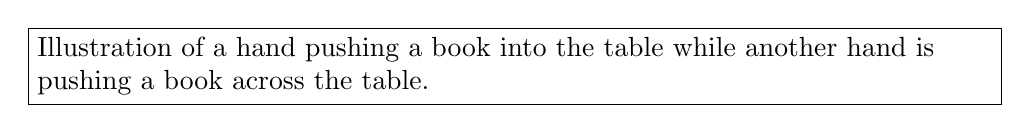
\begin{tikzpicture}
    \node[draw,align=left,text width=\textwidth] at (0,0) {Illustration of a hand pushing a book into the table while another hand is pushing a book across the table.};
  \end{tikzpicture}  
  \caption{Pushing a book into the table}
  \label{fig:perpendicularForce}
\end{marginfigure}

\subsection{Can work done be negative?}
Think about pushing a book across a table. The book moves forward because we apply a force. At the same time, the table exerts a friction force on the book in the opposite direction.

Remember that in formula for work (Equation \ref{eq:workDef}), distance $(d)$ is measured in the direction of the force. In this situation the book moves forward and the frictional force acts backward. So, the motion of the book is in the opposite direction to the friction force. When a force (like friction) tries to stop an object from moving forward, it is doing negative work because it is 'stealing' energy away from the motion.

If the force and the motion are in opposite directions, the work done is negative. Negative work does not mean “no work.” It means that the force is acting against the motion. It tries to slow the object down or stop it.

\newthought{Question:} We apply brakes to slow down and stop a cycle. The cycle is moving forward, but the braking force acts backward. Is the work done by the braking force positive or negative?

\section{Energy}
Energy is the capacity to do work. Let us understand this with an example. Imagine a stack of books kept on the floor. Let us pick up some of the books and place them on a table. To do this, we apply an upward force and move the books through a certain height. So, we have done work.

When we do work on the books, we are also transferring energy to them. The books on the floor have less energy than the books on the table that are at a higher position.

Similarly, imagine a football resting on the ground. It is not moving. When we kick the ball, we are applying a force to it over a short distance. So, we do work on the ball. As a result, energy is transferred from our body to the ball. This energy makes the ball move forward.

If we kick the ball harder, we are applying a larger force. So, we are doing more work, and more energy is transferred to the ball. The ball then moves faster and travels a longer distance. If the ball slows down and stops after some time, it is because forces like friction act on it and remove energy from it. In this way, by kicking the ball, we can clearly see how doing work transfers energy and causes motion.

\subsection{Relationship between work and energy}
Work and energy are closely related. When we do work on an object, we transfer energy to it. When an object does work on something else, it transfers energy from itself. Energy transferred to the object is positive work, and energy transferred from the object is negative work.

Work done on an object, its energy changes. We can say that work done on an object is the change in its energy. 
\begin{equation}
  \text{Work done on an object} = \text{change in the energy of the object}.  
\end{equation}
This means, if positive work is done, the energy of the object increases and if negative work is done, the energy of the object decreases. This idea is true even when the force is not constant or changes during motion.

The SI unit of both work and energy is the $(\unit\joule)$.

Our body gets energy to do work from the food we eat. The energy stored in food is often measured in calories (cal). 
\begin{equation}
1~cal = 4.2~\unit\joule. 
\end{equation}
\newthought{Exercise:} Look at the labels of packaged food items in your house. Write down the energy (in calories) given on each label.

\marginnote{James Prescott Joule studied how mechanical energy and heat (thermal energy) are related and how one can change into the other. His work showed that different forms of energy are connected, helping scientists develop a unified understanding of energy.

He carried out careful experiments on heat and discovered how heat is produced when an electric current flows through a conductor. This relationship is known as Joule's law of heating.

Joule's work played an important role in the development of thermodynamics, the study of heat and energy.

In recognition of his contributions, he was elected a Fellow of the Royal Society in 1850. The SI unit of energy, the joule (J\unit\joule), is named in his honor.
}

\begin{marginfigure}
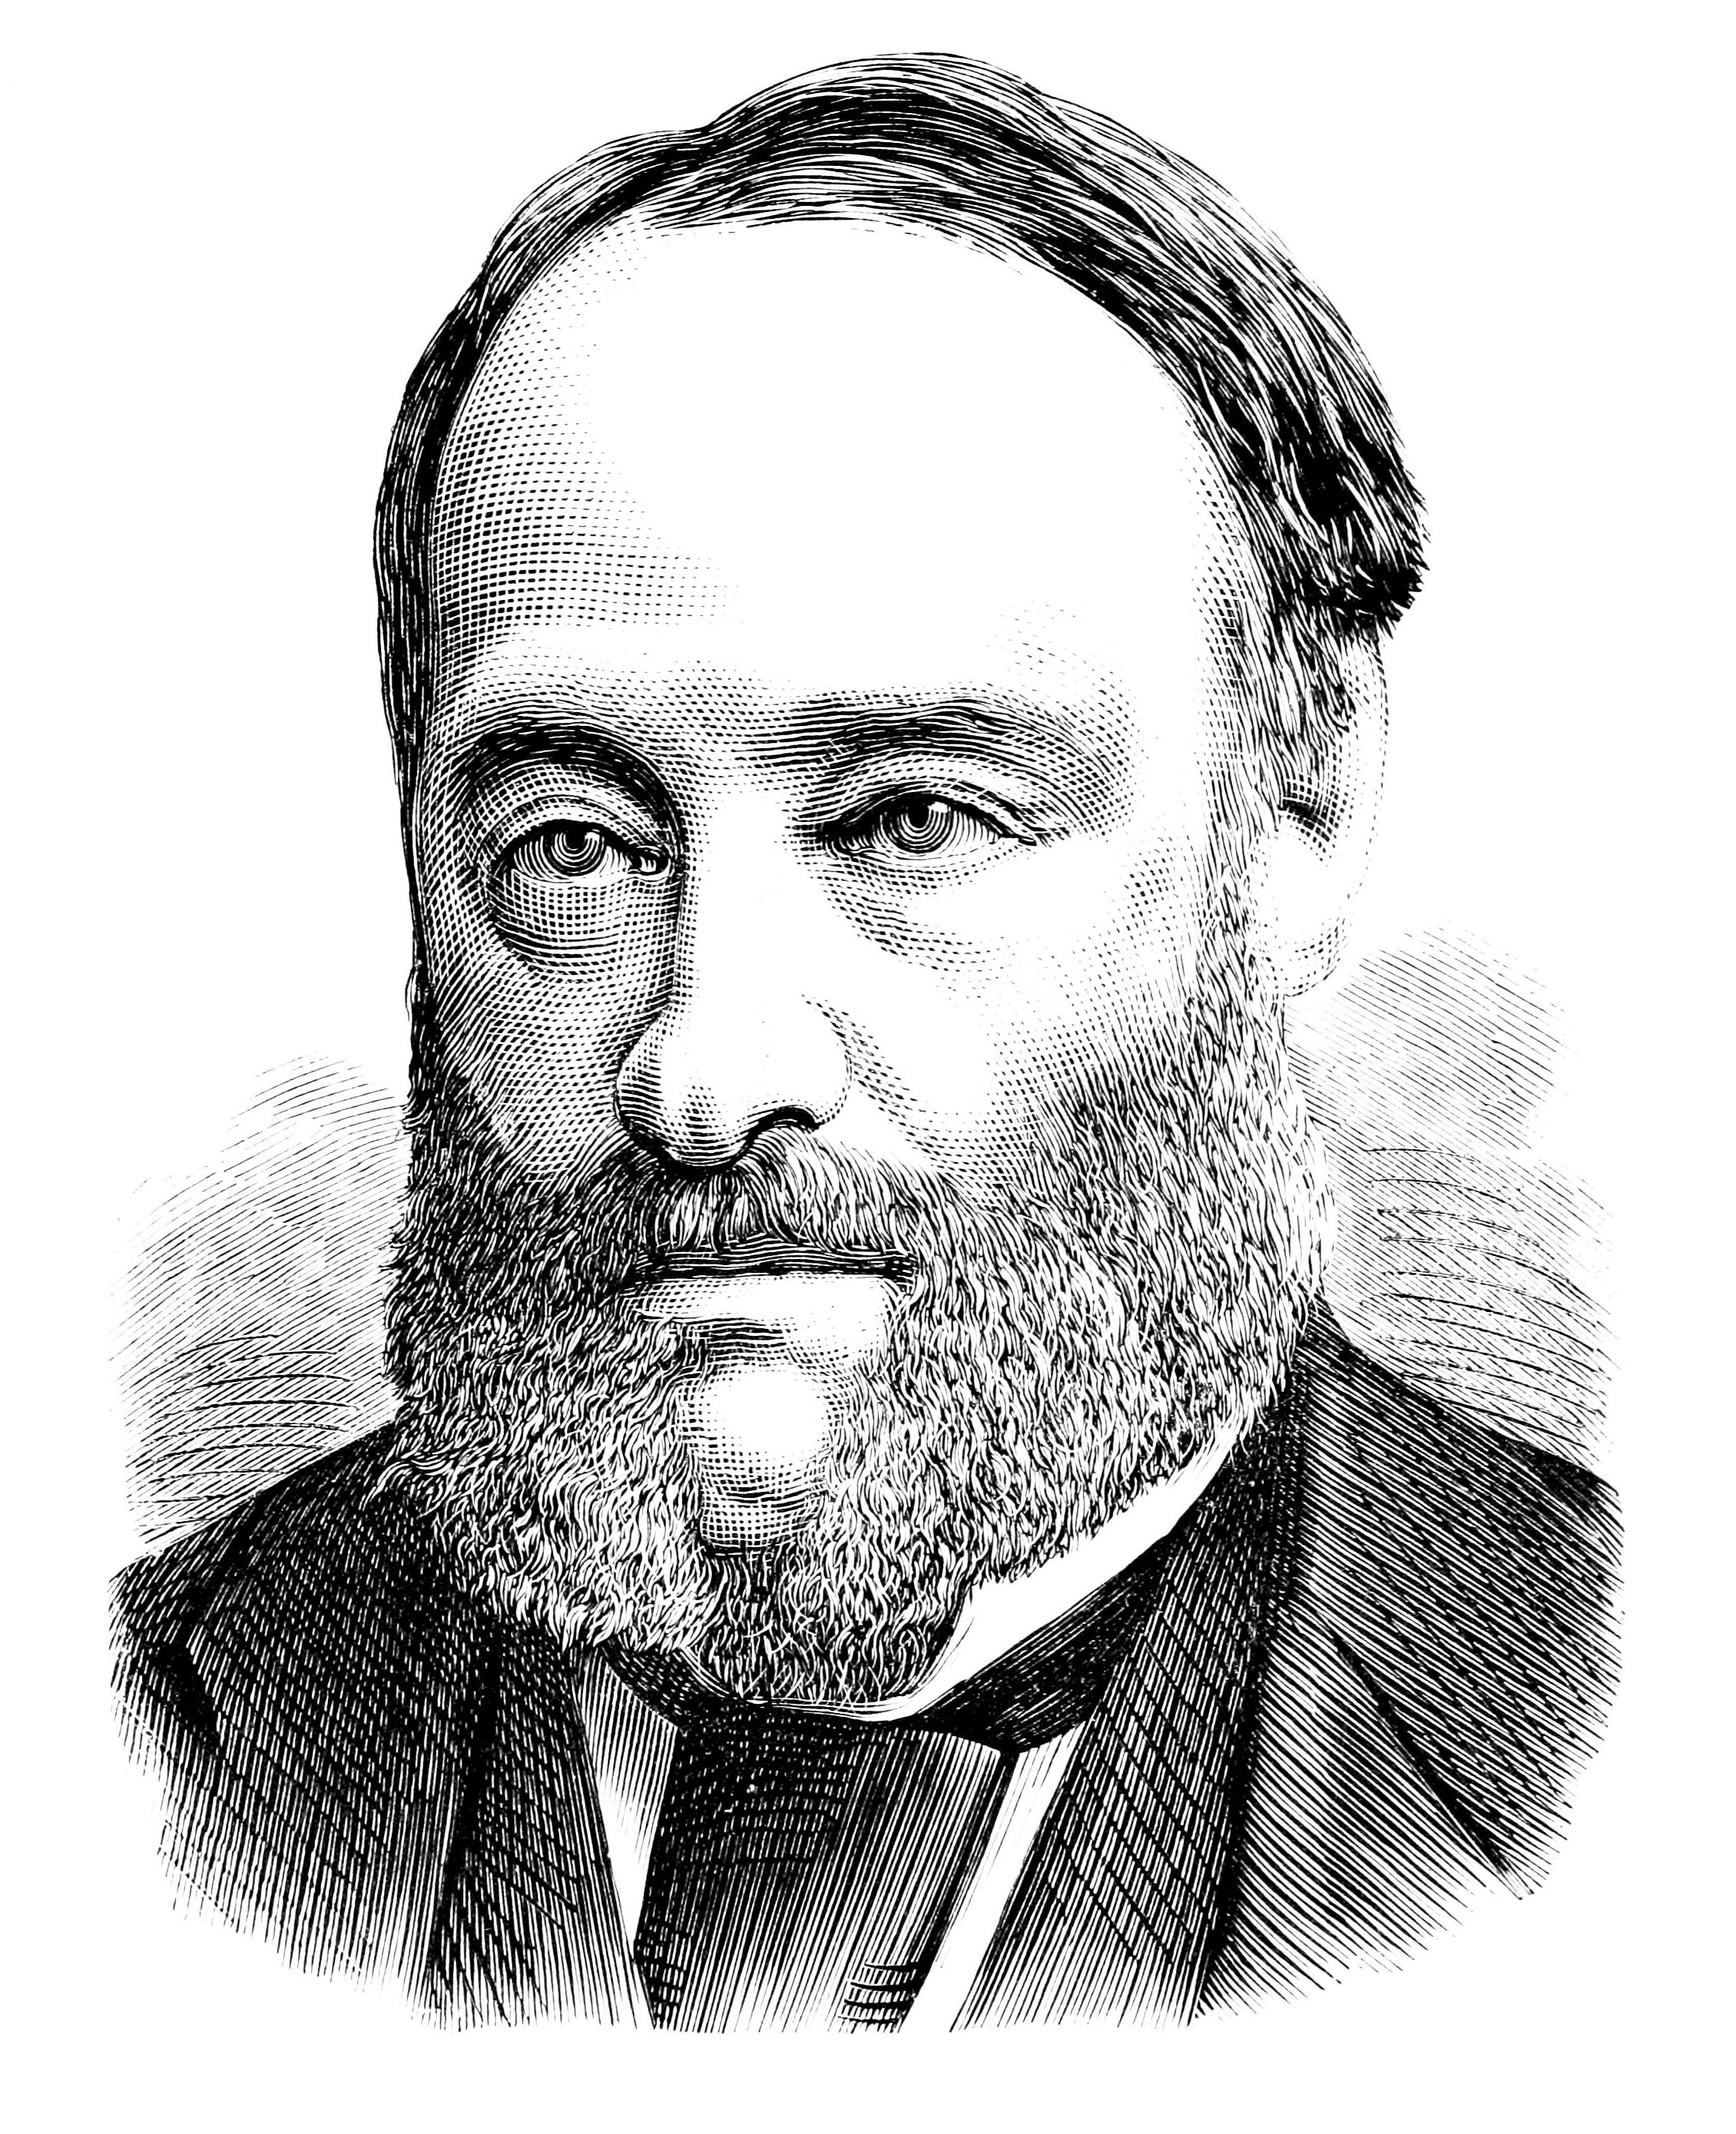
\includegraphics{PSM_V05_D008_James_Prescott_Joule} 
  \caption{James Prescott Joule}
\end{marginfigure}

\subsection{Different forms of Energy}
Energy can exist in many different forms. We do not always see energy directly, but we can observe its effects.

For example, the books placed on a table have more energy than the books on the floor. This energy depends on their position. It is called \textbf{potential energy}. 

Now imagine you push one of the books off the table. As the book falls, it starts moving. This energy due to motion is called \textbf{kinetic energy}. While the book is falling, its potential energy decreases and its kinetic energy increases. Just before it reaches the ground, most of its energy is in the form of kinetic energy. In this way, energy can change from potential energy to kinetic energy. Both potential energy and kinetic energy are forms of mechanical energy. \textbf{Mechanical energy} is the energy an object has due to its position or its motion.

In dam projects, water is stored at a height. This water has potential energy. When the water is released, it flows downward and gains kinetic energy. The moving water turns large turbines, which generate electricity. In this way, the energy of water is converted into electrical energy.
\begin{marginfigure}
  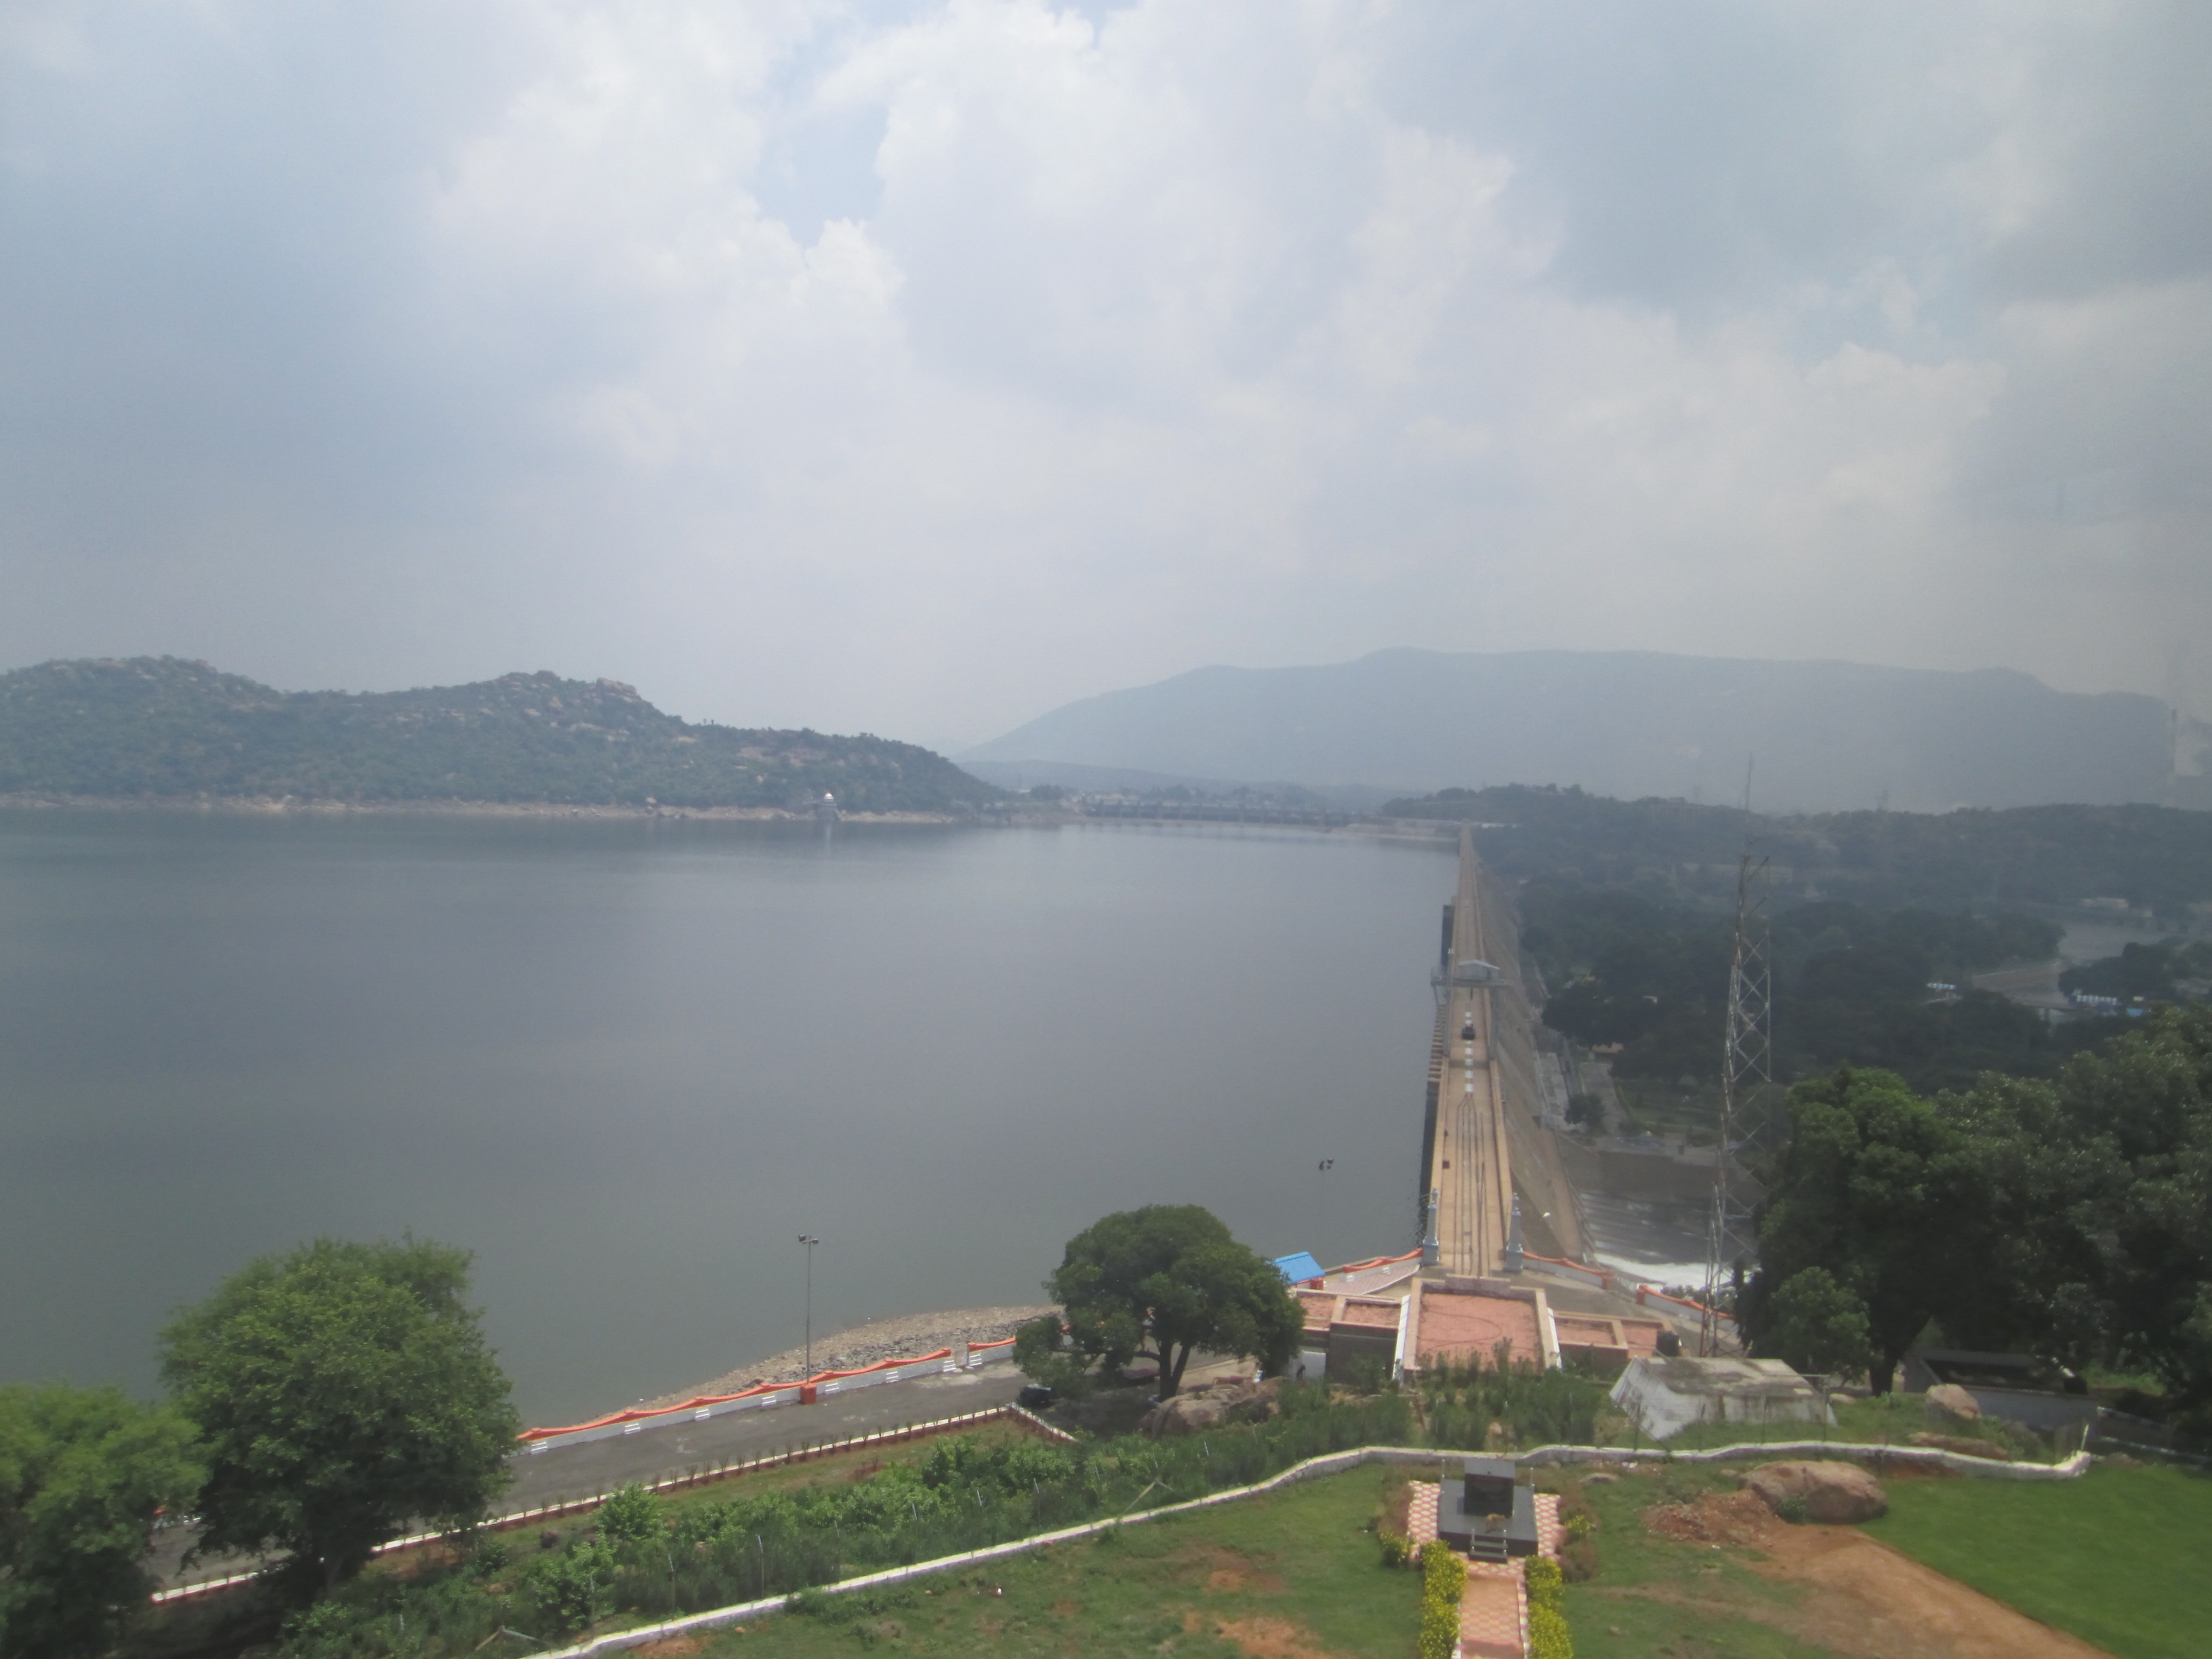
\includegraphics{Dam_Aerial_View}
  \caption{Mettur Dam located across the river Kaveri in Salem.}
\end{marginfigure}
In an electric circuit, energy is stored in a battery. This is \textbf{electrical energy}. When the bulb glows, electrical energy is converted into \textbf{light energy} and some energy is also converted into heat.

In your electricity bill, you are charged for the electrical energy you use. This is measured in kilowatt-hour (\unit{\kilo\watt\hour}).
\begin{equation}
  1~\unit{\kilo\watt\hour} = 3.6\times10^6 \unit{\joule}
\end{equation}

\newthought{Question:} Check your home electricity bill. How many units (\unit{\kilo\watt\hour}) of energy have you used? Provide your answer in the unit of Joule.

You may notice that when the electricity consumed at home is written in the unit of Joule, it is a large number. Measuring the electrical energy consumption in Joule is like measuring the distance between two cities in millimetre. Kilowatt-hour (\unit{\kilo\watt\hour}) is therefore a more convenient unit to measure electrical energy.

When we use an electric kettle electrical energy comes from the power supply. This energy passes through a metal coil (heating element) inside the kettle. The coil gets hot. This heat is transferred from the coil to the water. As a result, the temperature of the water increases and it eventually boils. The hot water has \textbf{thermal energy}.

When we beat a drum we use mechanical energy (movement of our hand). This energy is converted into \textbf{sound energy}. Similarly, speakers use electrical energy to produce sound.

The food we eat and fuels like petrol and gas store energy in the form of \textbf{chemical energy}. When we eat food, our body uses this energy to move, work, and stay warm. When fuel burns, chemical energy is released as heat and light.
\begin{marginfigure}
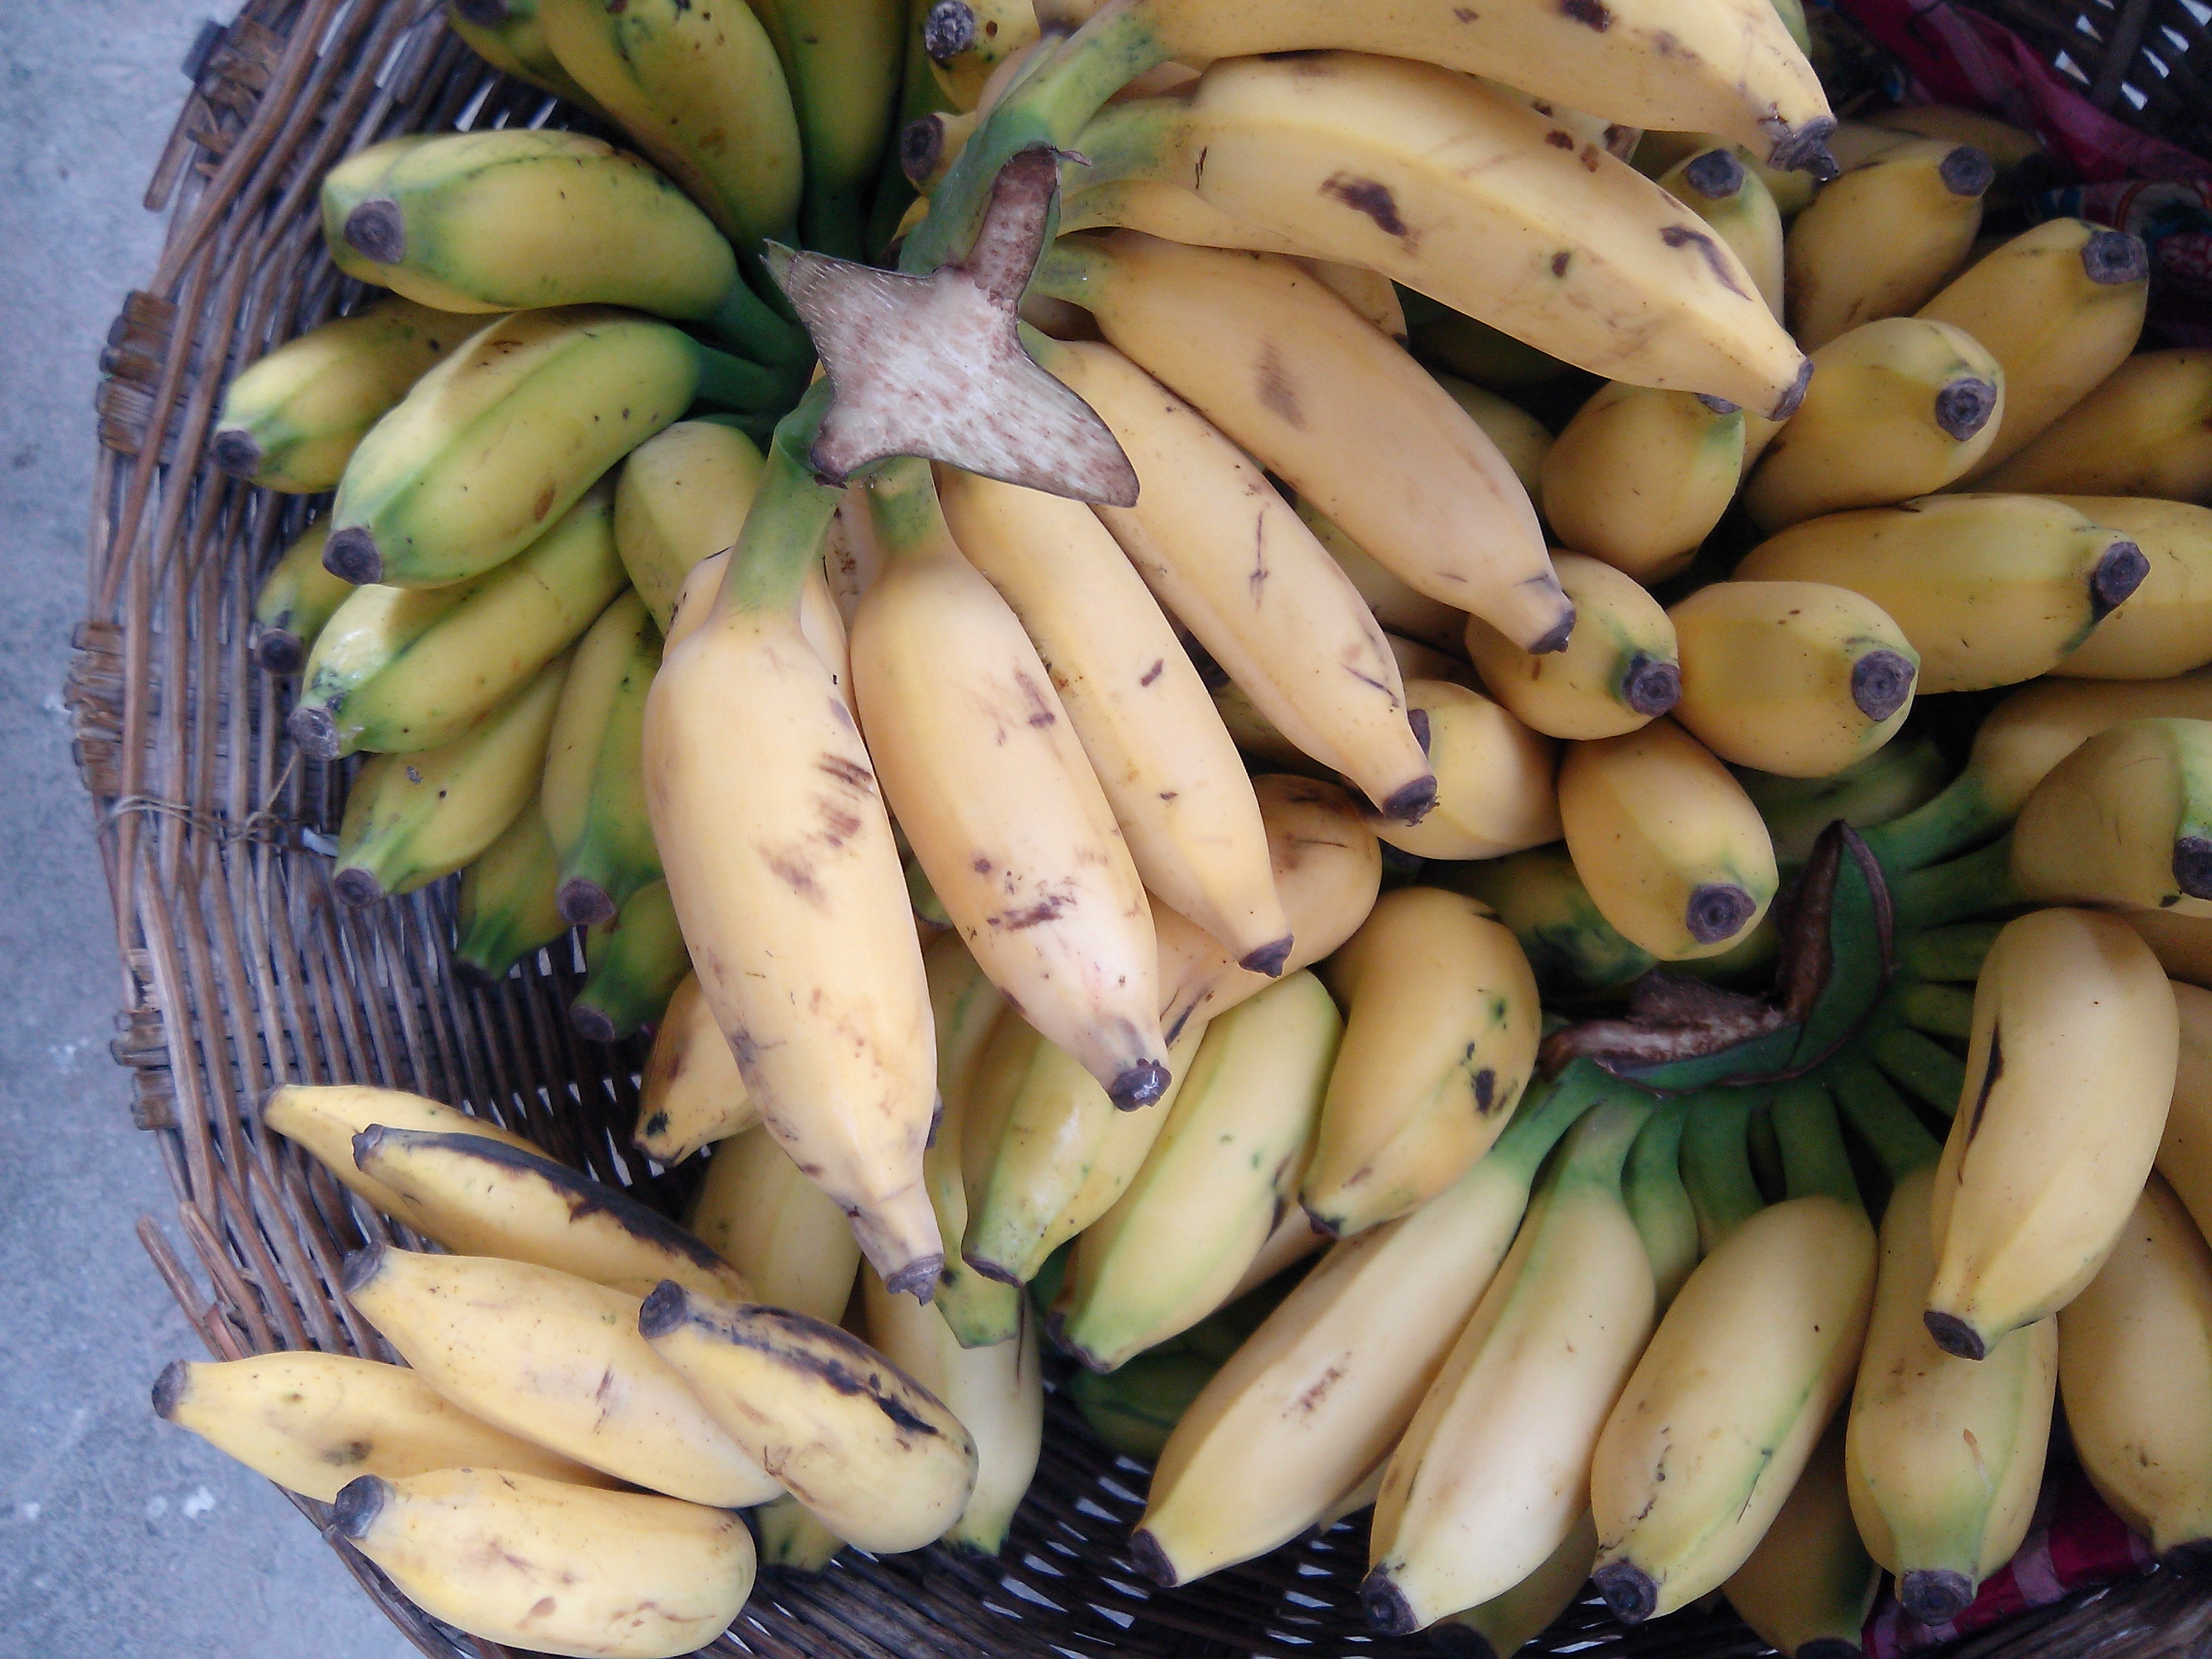
\includegraphics{Salem_Palaintains_of_Tamil_Nadu}
  \caption{Every 100~\unit\g of banana contains apporximately 89 calories of energy.}
\end{marginfigure}
\newthought{Question:} A banana contains 100 calories of energy. How much energy is this in joules?

Energy is also stored inside the nuclei of atoms. This is called \textbf{nuclear energy}. It is released in special processes and is used, for example, to generate electricity in nuclear power plants. Nuclear energy powers the Sun. 
\begin{marginfigure}
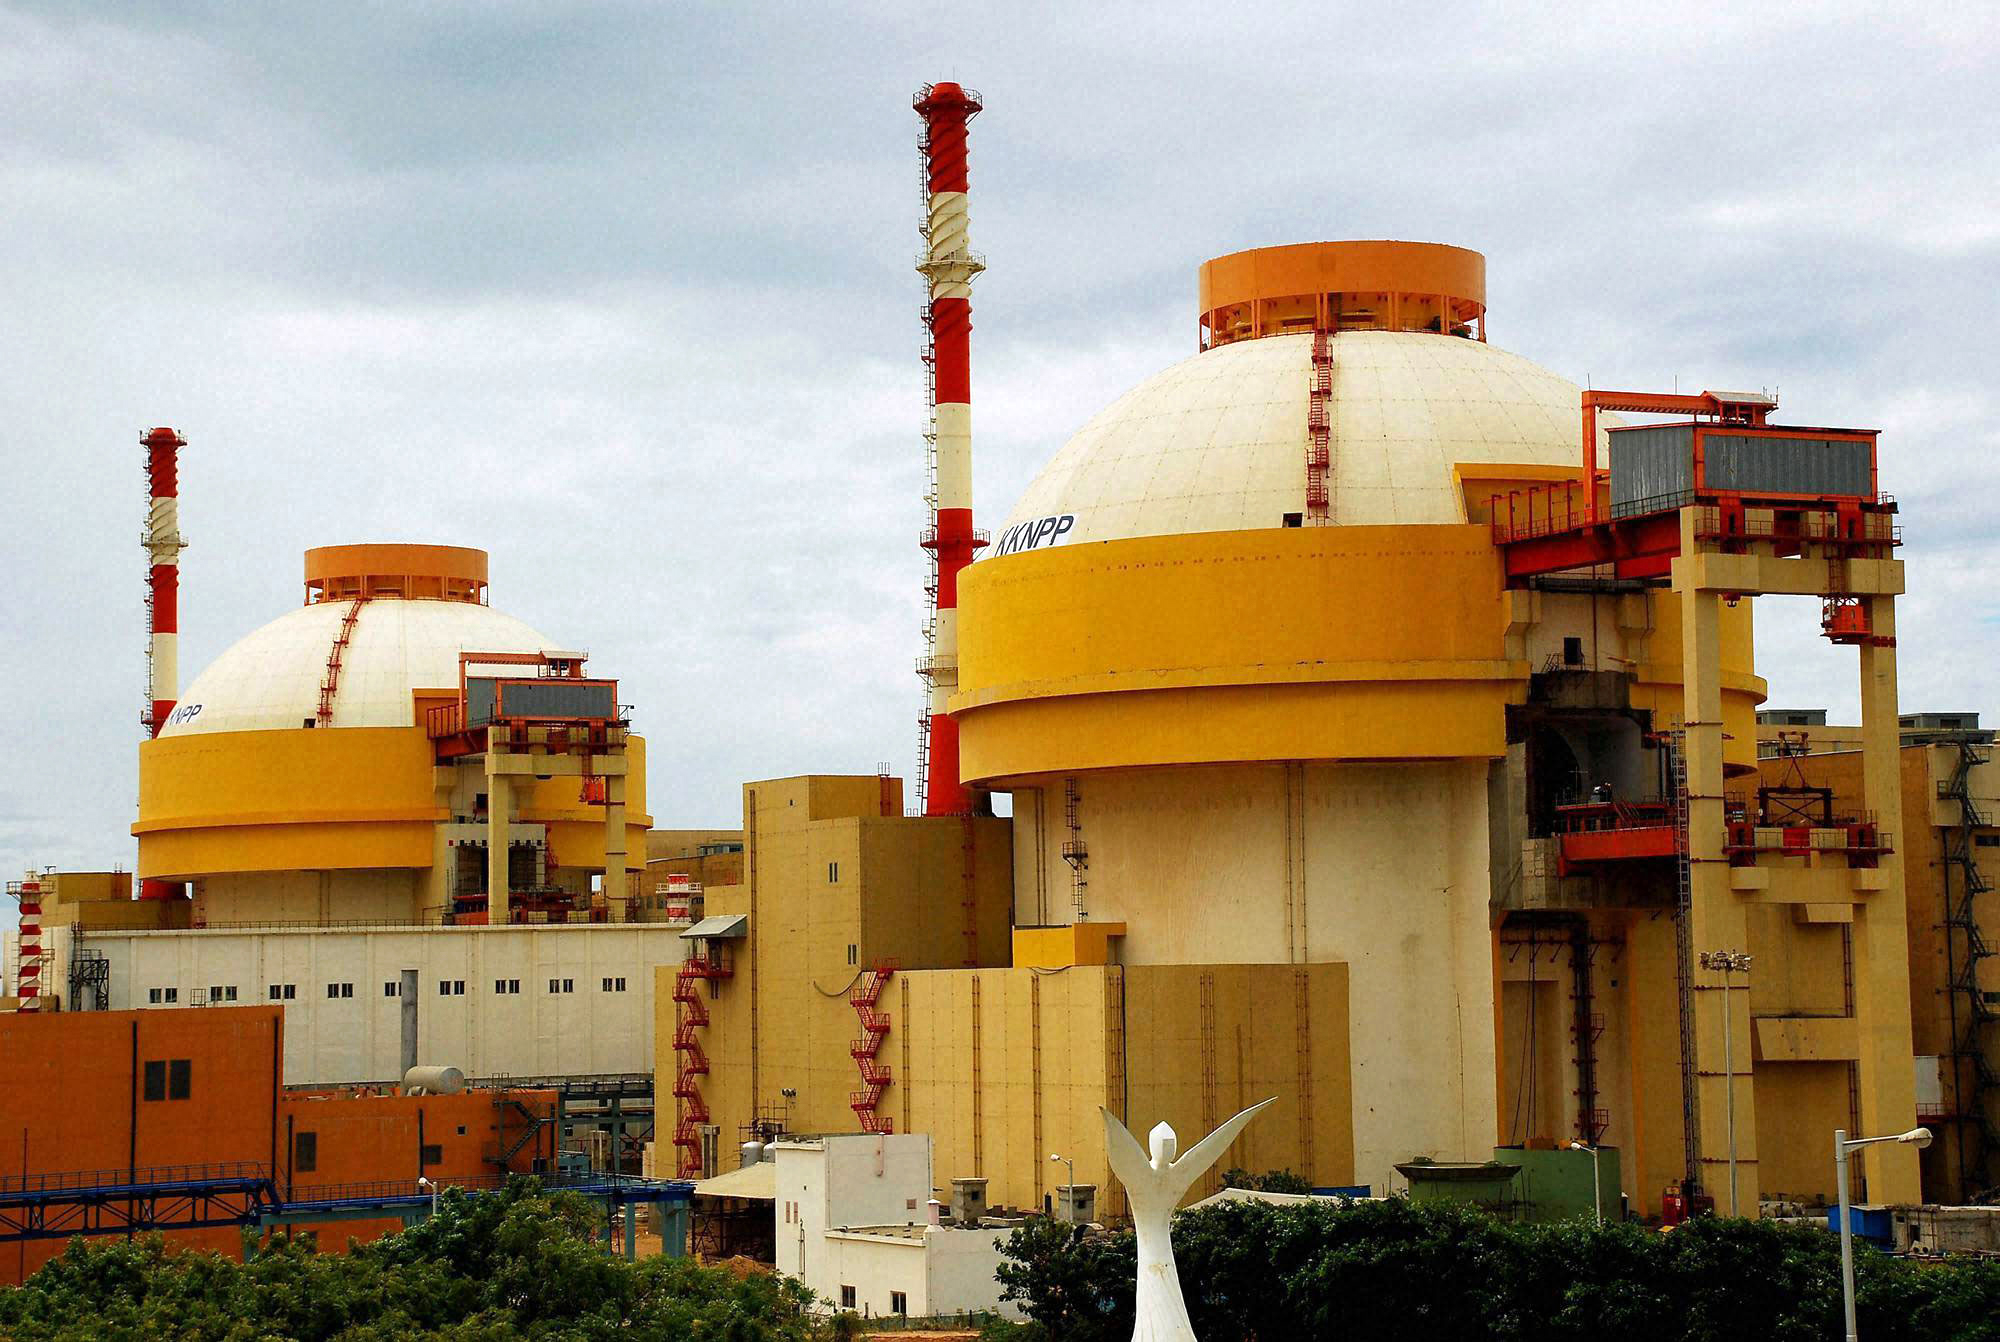
\includegraphics{KKNPP_PTI}
  \caption{Kudankulam Nuclear Power Plant in Tirunelveli}
  \label{fig:perpendicularForce}
\end{marginfigure}

Energy can change from one form to another. It does not disappear. When we observe any activity around us, we can often trace how energy changes form step by step.

For example, when you eat food and then run, the energy stored in the food (chemical energy) is used by your muscles to produce motion. Some of this energy also changes into heat, which keeps your body warm.

In another example, sunlight falls on wet clothes. The energy from sunlight is transferred to the water in the clothes. This energy makes the water evaporate, and the clothes dry.

Similarly, when you switch on a torch, the battery provides electrical energy. This energy is converted into light (and some heat), which helps us see in the dark.

In each of these cases, energy is not lost. It only changes from one form to another.

\newthought{Exercise:} Choose one of the examples above and draw arrows to show how energy changes form.
Example: Food $\to$ muscle $\to$ motion $\to$ heat

\newthought{Question:} When you ride a cycle, what forms of energy are involved?
\newthought{Question:} When a fan is running, how does energy change form?

\subsection{Law of Conservation of Energy}
Energy can change from one form to another, but the total amount of energy remains the same. This idea is called the \emph{Law of Conservation of Energy}.

Consider a roller coaster. When the coaster is at the top of a track, it has high potential energy because of its height. As it moves down, this potential energy changes into kinetic energy, and the coaster speeds up. When it climbs up again, kinetic energy changes back into potential energy, and the speed decreases.

\begin{marginfigure}
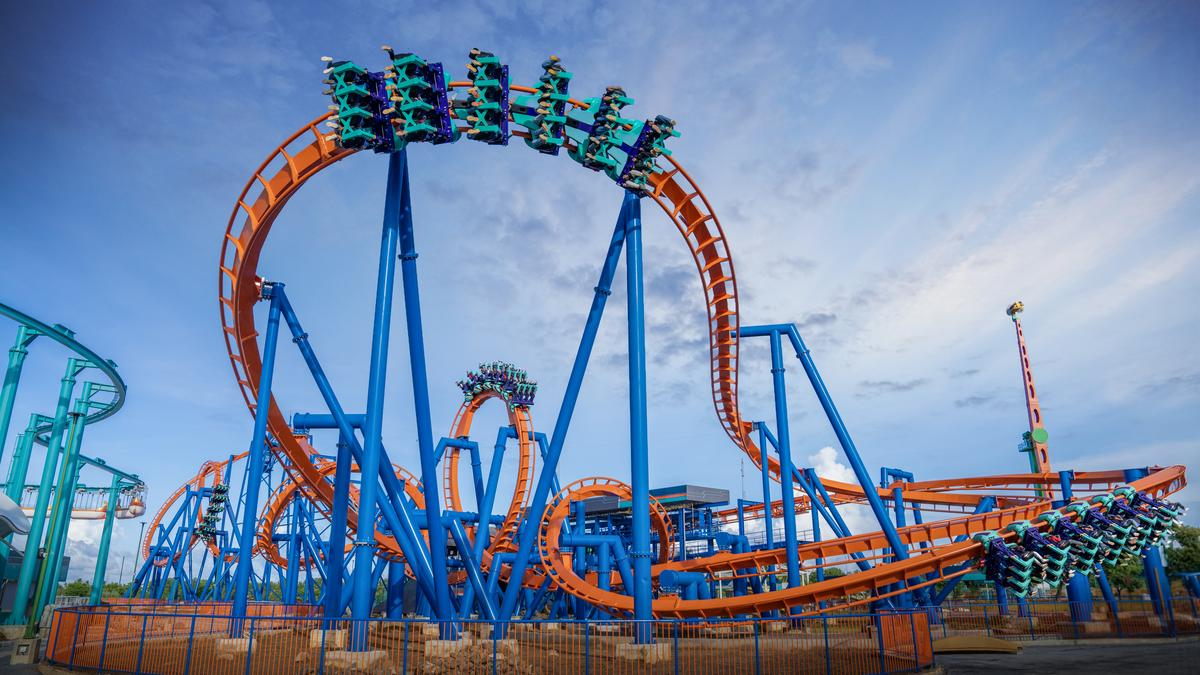
\includegraphics{WonderlaChennai2}
  \caption{Roller coaster in a theme park in Chennai.}
\end{marginfigure}

In a similar way, think about riding a bicycle down a slope. At the top, you have more potential energy. As you move down, this changes into kinetic energy and you go faster. When you go up another slope, your speed decreases as kinetic energy changes back into potential energy.

In all these cases, energy is not lost. It only changes from one form to another. The total energy remains constant.

\newthought{Exercise:}
Complete the table below. For each situation, describe what is happening and identify the form of energy before and after the change.

\begin{table}[h]
  \centering
  \fontfamily{ppl}\selectfont
  \begin{tabular}{p{0.2\textwidth}p{0.2\textwidth}p{0.2\textwidth}p{0.2\textwidth}p{0.2\textwidth}} 
    \toprule
    What is happening? & Where is energy at the start? & Form of energy (before) & Form of energy (after) & Where does the energy go to?\\
    \midrule
    We push a book and it moves &body & chemical energy & kinetic energy & book \\
    \bottomrule    
    \ldots &\ldots & \ldots & \ldots & \ldots \\    \bottomrule
    \ldots &\ldots & \ldots & \ldots & \ldots \\    \bottomrule
    \ldots &\ldots & \ldots & \ldots & \ldots \\    \bottomrule
    \ldots &\ldots & \ldots & \ldots & \ldots \\    \bottomrule
  \end{tabular}
  \label{tab:energy-table}
  %\zsavepos{pos:normaltab}
\end{table}
\subsection{Energy from the Sun}
The Sun is an important source of energy for life on Earth. It gives us light energy and heat energy.

We use sunlight in many ways. We use it for drying washed clothes. Plants use sunlight for photosynthesis to grow. Plants later becomes our food.  Sunlight is a renewable source of energy. This means it is naturally available and will not run out in a short time.

\begin{figure}[h]
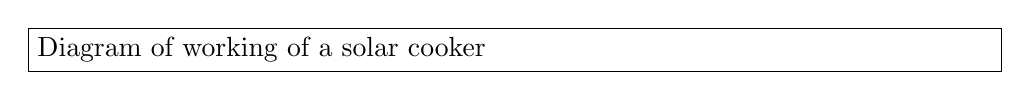
\begin{tikzpicture}
    \node[draw,align=left,text width=\textwidth] at (0,0) {Diagram of working of a solar cooker};
  \end{tikzpicture}  
  \caption{A solar cooker uses sunlight and can be used on a sunny day to cook food. A solar cooker does not use fuel like gas or coal. It does not produce smoke. It helps reduce energy waste.}
\end{figure}

Sunlight, wind and flowing water are examples of renewable energy sources. These sources can be used again and again. Hydroelectric power and power generated from wind turbines are a renewable source of energy because it depends on the natural water cycle and flowing wind. 
\begin{figure}[h]
  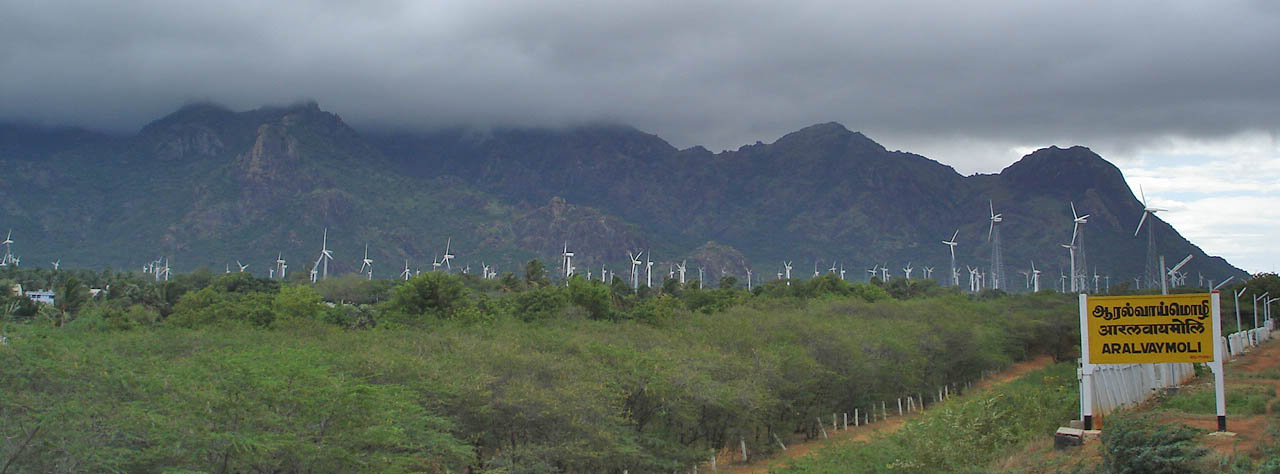
\includegraphics{Aralvaimozhy_station}
  \caption{The largest wind farm of India in Muppandal, Kanyakumari.}
\end{figure}
\begin{marginfigure}
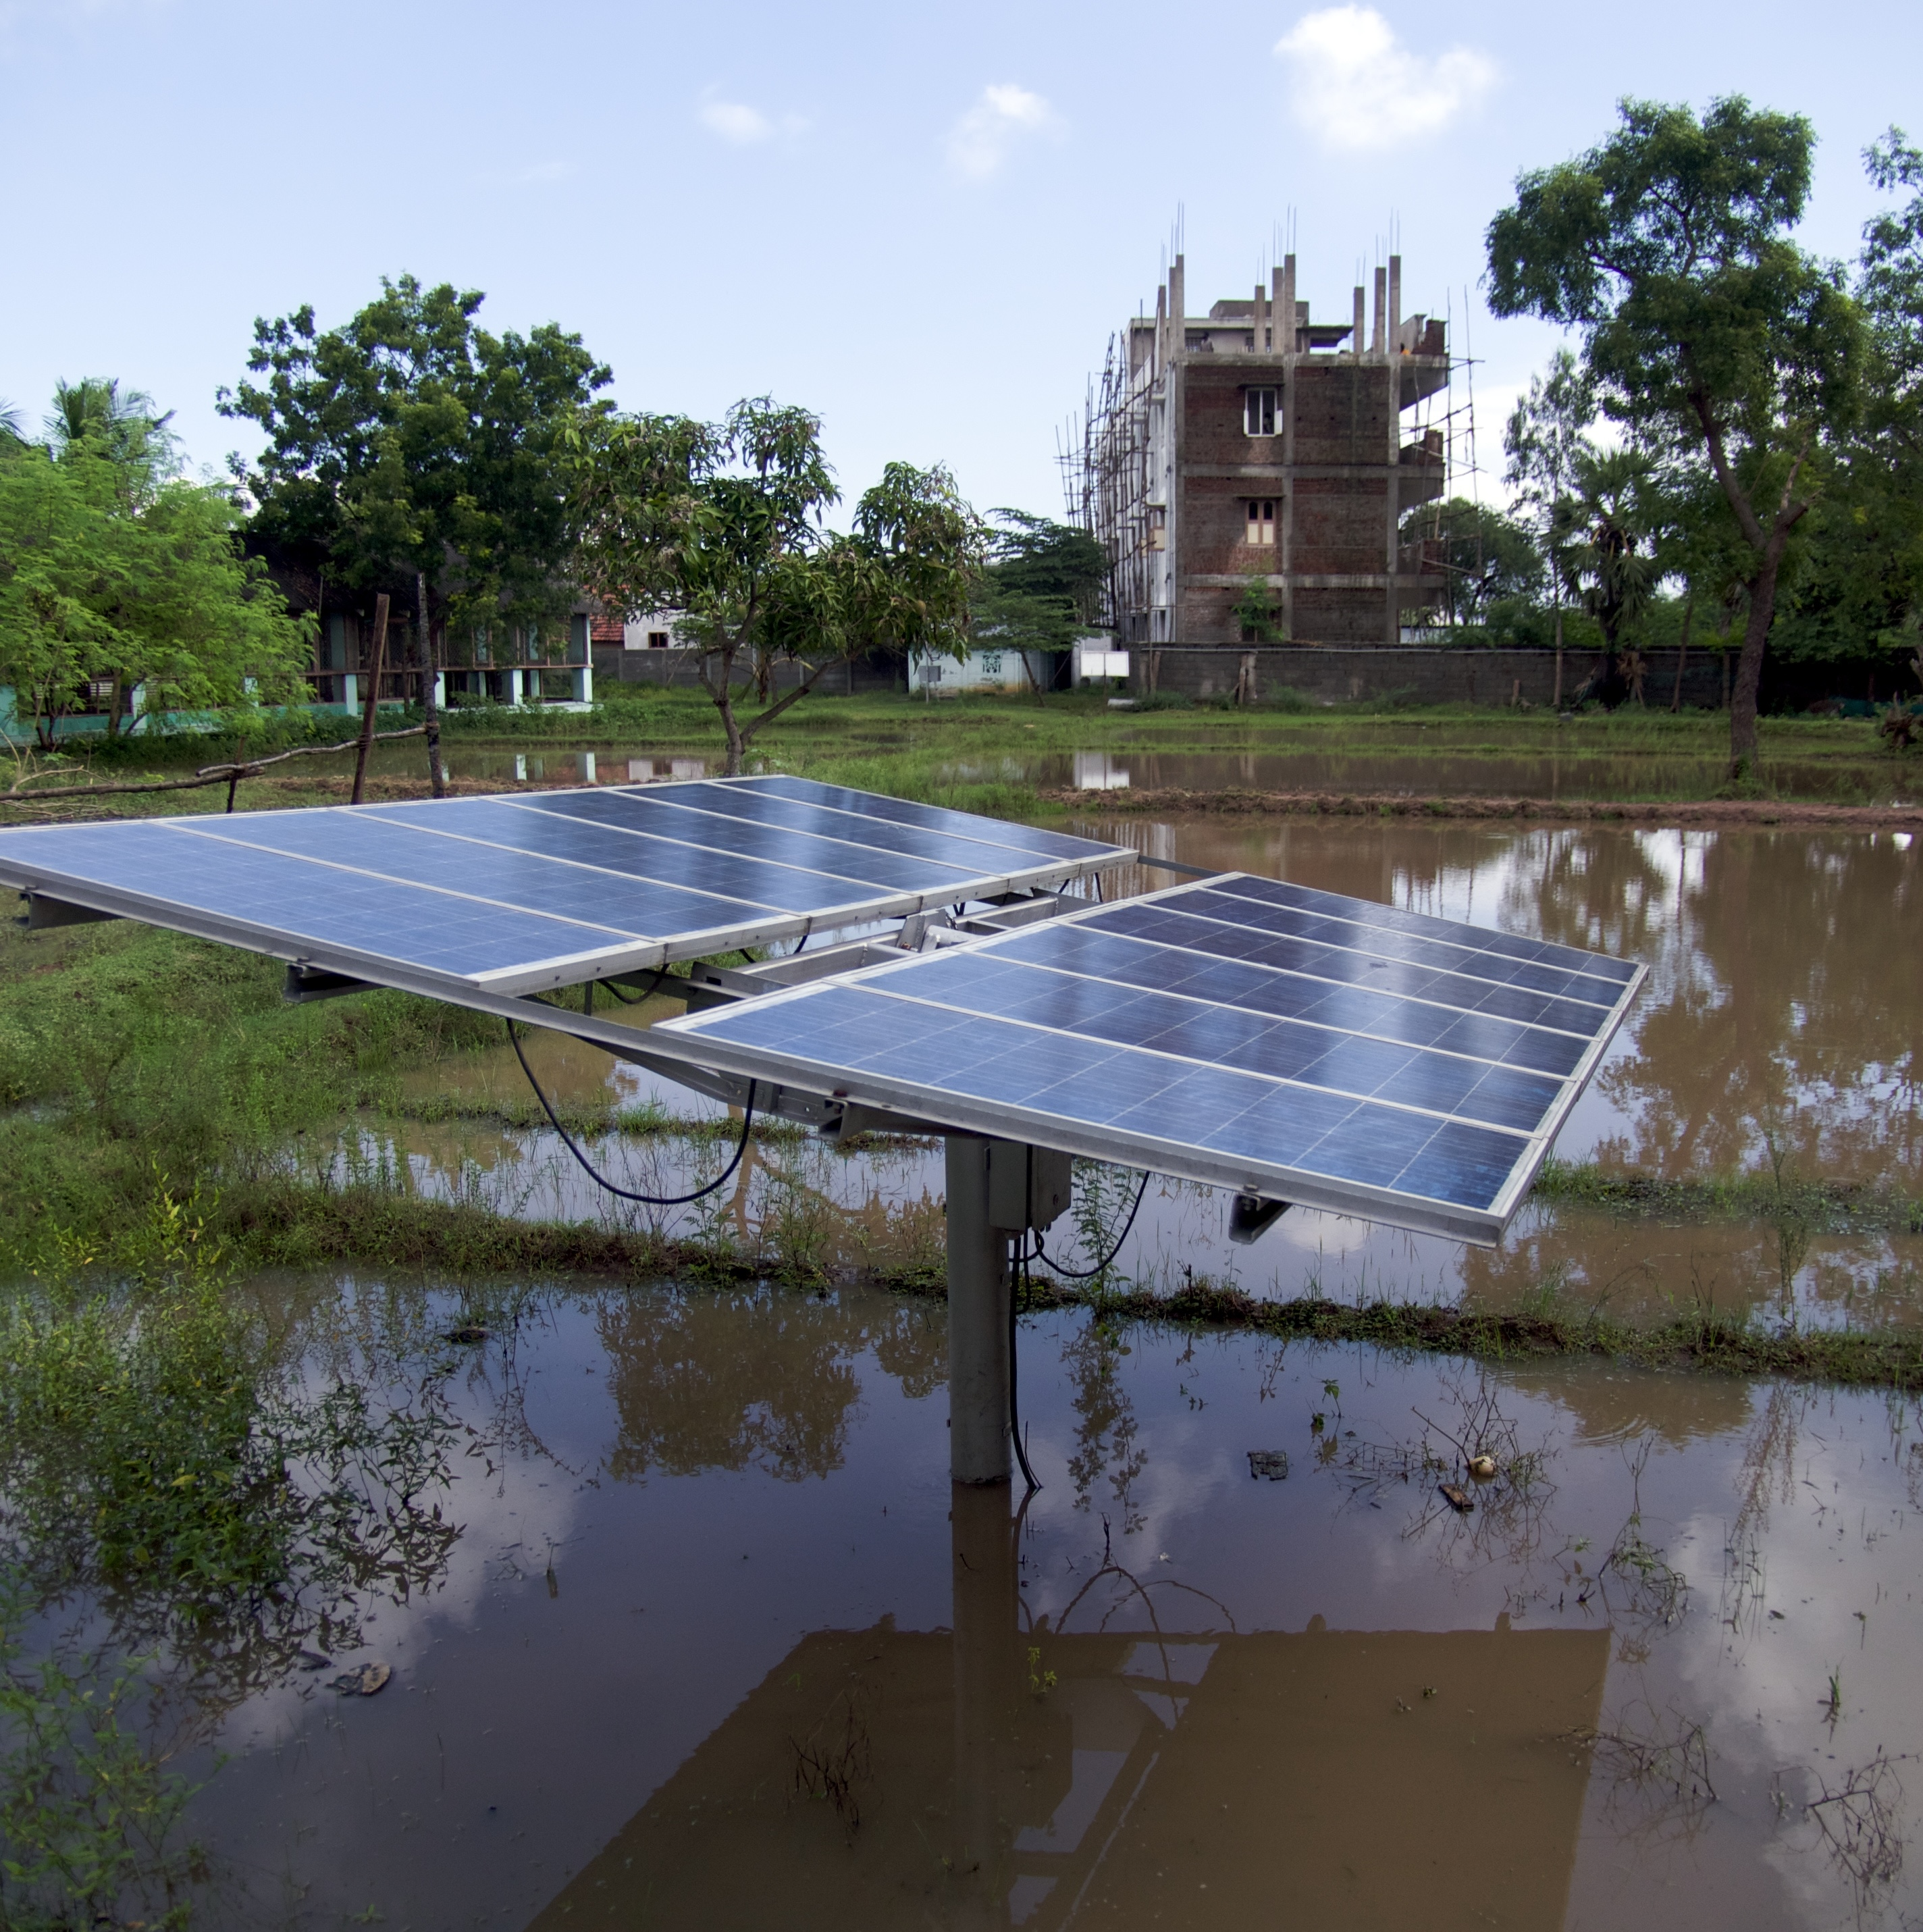
\includegraphics{Solar_Panels_in_Farm,_India}
\caption{A farm in which uses Solar Power to run its water pumps and lights.}
\end{marginfigure}
Coal, petrol, and natural gas are non-renewable energy sources. Non-renewable energy sources take millions of years to form and can get used up.

Energy from non-renewable sources is limited. If we waste it, it may not be available in the future. Using renewable sources and reducing unnecessary use helps save energy.

\newthought{Question:} Give one real-life situation where understanding energy can help reduce waste.
Example: Switching off lights and fans when not in use to save electrical energy.

\newpage
\section{Image Source}
\begin{table}[h]
  \centering
  \fontfamily{ppl}\selectfont
  \begin{tabular}{p{0.3\textwidth}p{0.5\textwidth}p{0.2\textwidth}} 
    \toprule
    Figure & Source & License\\
    \midrule
    Roller coaster in a theme park in Chennai. &\url{https://th-i.thgim.com/public/incoming/8sgztp/article70344934.ece/alternates/LANDSCAPE_1200/Wonderla%20Chennai%20%202.jpg} & Copyright Wonderla Chennai \\
    \bottomrule      
 The largest wind farm of India in Muppandal, Kanyakumari. & \url{https://commons.wikimedia.org/wiki/File:Aralvaimozhy_station.jpg#/media/File:Aralvaimozhy_station.jpg} & CC-by-sa
PlaneMad/Wikimedia\\
    \bottomrule    
A farm in which uses Solar Power to run its water pumps and lights. & \url{https://commons.wikimedia.org/wiki/File:Solar_Panels_in_Farm,_India.jpg#/media/File:Solar_Panels_in_Farm,_India.jpg} & CC BY 2.0\\
    \bottomrule  
    Mettur Dam located across the river Kaveri in Salem & \url{https://commons.wikimedia.org/wiki/File:Dam_Aerial_View.JPG#/media/File:Dam_Aerial_View.JPG} & CC BY-SA 4.0\\
    \bottomrule  
    Every 100~\unit\g of banana contains apporximately 89 calories of energy. & \url{https://commons.wikimedia.org/wiki/File:Salem_Palaintains_of_Tamil_Nadu.jpg#/media/File:Salem_Palaintains_of_Tamil_Nadu.jpg} & CC BY-SA 4.0\\
    \bottomrule  
    James Prescott Joule & \url{https://commons.wikimedia.org/wiki/File:PSM_V05_D008_James_Prescott_Joule.jpg#/media/File:PSM_V05_D008_James_Prescott_Joule.jpg} & Public Domain\\
    \bottomrule  
    Figure & Source & License\\
    \bottomrule  
        Figure & Source & License\\
    \bottomrule  
        Figure & Source & License\\
    \bottomrule  
        Figure & Source & License\\
    \bottomrule  
  \end{tabular}
\end{table}
\nocite{halliday2013fundamentals}
\nocite{walker2006flying}

\bibliographystyle{plainnat}
\bibliography{workandenergy}
\end{document}

Where does the energy go when a moving object stops? For example, when you throw a ball up, it moves, has kinetic energy by virt, 

> A ball rolls, slows down, and stops.
> Has energy disappeared?

Question: Tracking energy

 Situations

1. Falling object
2. Cycling and braking
3. Electric fan
4. Boiling water

 Task (worksheet)

Fill:
(also provide an example)
| Step | What happens | Energy form before | Energy form after |
| ---- | ------------ | ------------------ | ----------------- |
 
Energy changes form, it does not just vanish. 


Question: Design a system that uses energy usefully”

Examples:

Solar cooker

Identify source of energy, Show transformations, Explain how waste is reduced

Question: One situation where understanding energy can help reduce waste.

Strait of Hormutz
Energy crisis
Efficient use of energy

Energy is associated with state (of motion, position)
temperature (motion of molecule) do we mention this? shall we restrict to kinetic energy only?

conserved

can be changed from one form to another (like money)

kinetic energy

potential energy, while cycling uphill is difficult, need to put more energy to peddle

Roller coaster during fairs, how do they work?



Suddenly you realize that a car is headed toward your car the
wrong way in a one-way tunnel. To minimize your danger
from the impending accident, should you match your speed
to that of the other car, go even faster, or slow to a stop?
A head-on collision is the most dangerous type of car col-
lision. Surprisingly, the data collected about head-on collisions
suggest that the risk (or probability) of fatality to a driver is less
if that driver has a passenger in the car. Why is that?

The best advice is to stop and, if possible, put
your car in reverse. You can get a measure of the severity of
the collision by considering the total kinetic energy or the
total momentum of the cars before the collision. If you do
not decrease your speed toward the other car, both quanti-
ties are large, and so the collision will be severe.
The situation is unlike football, where one player may
choose to speed up when running head-on into another
player. The difference is that a player may want the colli-
sion to be violent, and by properly orienting his body he
can shift the collision to his opponent's vulnerable area or
cause his opponent to become unbalanced and slam into
the field.
Data collected about head-on car collisions indicate that
adding a passenger to your car reduces your risk of fatality.
That risk depends on the change in your velocity during the
collision: A large change means that you undergo a severe
acceleration due to a severe force. For example, if your car has
a small mass and the other car has a large mass, your veloci-
ty may be changed so much that you end up going backward.
Additional mass in your car, from a passenger or even a sand-
bag in the trunk, can decrease your change in velocity and
thus also your risk. Here is one numerical result: Suppose
your car and the other car are identical and that your mass
and the other driver's mass are identical. Your fatality risk is
reduced by about 9% if you have an 80 kilogram passenger
in your car.


examples from cricket

newton's cradle

Why do balls bounce?

  Rock climbers (as opposed to spelunkers) use rope
that gives considerably under stress, so that if you fall, your
stop at the end of the fall is not sudden and the force stop-
ping you is not huge. As the rope begins to stretch, the rope
materials rub against one another and become warmer; most
of the potential energy and kinetic energy that you lose dur-
ing the fall ends up as thermal energy within the rope.

Playing carroms

Working of a yoyo -  when talking about types of mechanical energy

Playing using spinning tops